% Presenting ReaxFF
    \subsection{Présentation de \reaxff{}} \label{sec:reaxff}

\begin{figure}[h!]
    \centering
    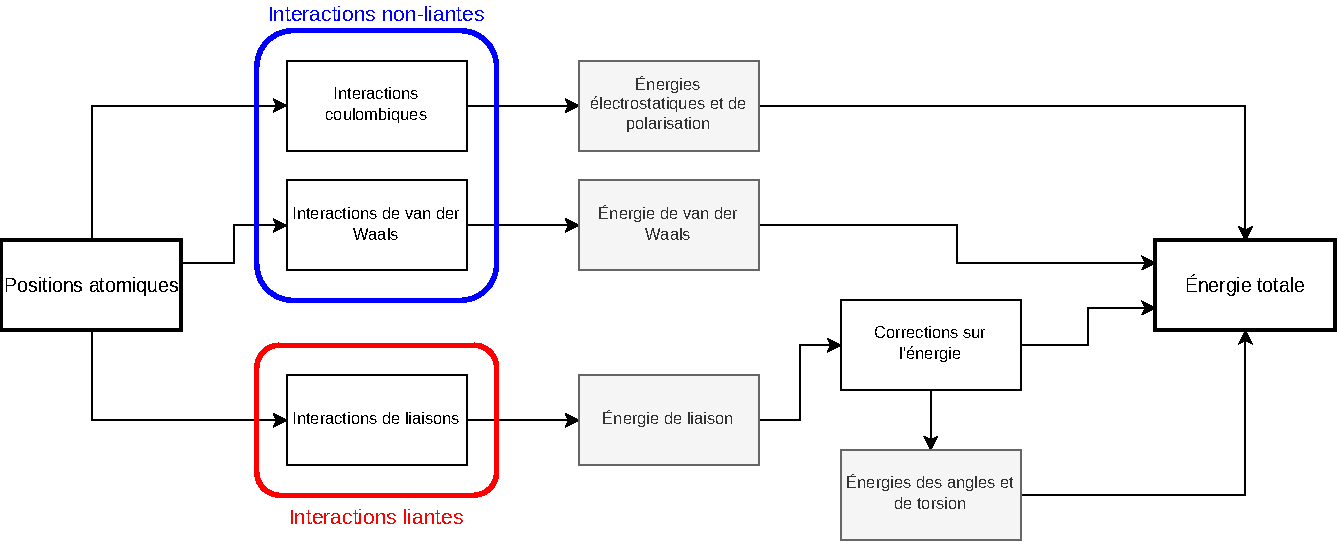
\includegraphics[width=\linewidth]{H2O-ReaxFF-interactions.pdf}
    \caption{Interactions et énergies au sein de \reaxff{} (tiré de \cite{russo_atomistic-scale_2011})}
    \label{fig:interactions_energies_reaxff}
\end{figure}

\reaxff{}\cite{russo_atomistic-scale_2011}\cite{senftle_reaxff_2016} est un potentiel utilisant les ordres de liaison pour modéliser des interactions atomiques en prenant aussi en compte les réactions chimiques (\autoref{fig:interactions_energies_reaxff}).\\
Il a été conçu de façon à obtenir des résultats dont la précision se rapproche des méthodes quantiques, en mettant en jeu autant d'atomes que les méthodes classiques.

Cette méthode se base sur le formalisme des ordres de liaison, où l'énergie d'une liaison entre un atome $i$ et un atome $j$ est donnée par :
\begin{equation}
    BO_{ij} = \exp \left[p_{bo, 1} \left(\frac{r_{ij}}{r_o}\right)^{p_{bo,2}}\right] + \exp \left[p_{bo,3} \left(\frac{r_{ij}^\pi}{r_o}\right)^{p_{bo,4}}\right] + \exp \left[p_{bo,5} \left(\frac{r_{ij}^{\pi\pi}}{r_o}\right)^{p_{bo,6}}\right]
    \label{eq:ordres_liaisons_reaxff}
\end{equation}
en s'appuyant sur un bon nombre de paramètres -- $p_{bo,1}, \dots, p_{bo,6}, r_o$ -- issus de calculs \textit{ab initio}, et dépendant de la nature des atomes mis en jeu, et du type de liaison considéré. Et pour les molécules, ce potentiel corrige l'énergie calculée pour l'utiliser lors du calcul des énergie d'angles, de torsions, etc..

Enfin, ce potentiel a été comparé à un modèle existant de la molécule d'eau à la \autoref{sec:h2o}.

% Presenting EChemDID
    \subsection{Présentation d'\echemdid{}} \label{sec:echemdid}
